% !TEX root = ../Thesis.tex

\chapter{Verzeichnis der KI-Nutzung}
\label{ch:ki-nutzung}

\input{content/00_KIErklaerung}

Tabelle~\ref{tab:ki-nutzung} listet alle in dieser Arbeit verwendeten KI-Werkzeuge auf.
\newpage


\section{Copilot Prompts für die unterstützende Systemanalyse von frag.jetzt}
\label{sec:anhang-copilot-prompts}

\begin{lstlisting}[caption={Copilot-Prompts zur Architekturanalyse}]
Analysiere die Projektstruktur von frag.jetzt. Welche Module, Services und Hauptkomponenten gibt es? Erstelle eine tabellarische Uebersicht mit Modulname, Technologie/Framework und Hauptverantwortung.
Identifiziere alle externen HTTP-Aufrufe (REST-Clients, WebClients, Feign-Clients) im Spring-Boot-Backend. Welche externen Dienste werden aufgerufen, mit welchen Endpunkten, und gibt es Timeout- oder Retry-Konfigurationen?
Liste alle REST-Controller im Backend auf. Gruppiere sie nach fachlicher Funktion (z. B. Room-Management, Question-Management, Auth, AI-Service) und notiere die HTTP-Methoden und Pfade.
Gibt es bereits Observability-bezogene Konfigurationen? Suche nach: Micrometer, Actuator, OpenTelemetry, Prometheus, Logging-Frameworks (Logback, Log4j), Health-Check-Endpoints, Tracing-Bibliotheken.
Analysiere die Datenbankschicht. Welche Entities/Tabellen gibt es, welche Repositories werden verwendet, und gibt es komplexe Queries oder Stored Procedures, die als Performancerisiko gelten koennten?
Beschreibe die WebSocket-Kommunikation. Welche STOMP-Topics oder Channels gibt es, welche Nachrichten werden darueber ausgetauscht, und wie wird die Verbindung verwaltet?
Analysiere die Deployment-Konfiguration (docker-compose.yml, Kubernetes-Manifeste, CI/CD-Pipeline). Welche Container/Services werden deployt, wie sind sie vernetzt, und welche Ressourcenlimits sind konfiguriert?
\end{lstlisting}
\newpage

% Ausgelagerte Landscape-Tabelle für das Verzeichnis der KI-Nutzung
% Header-Linie für Landscape-Seiten deaktivieren
\KOMAoptions{headsepline=false}%
\begin{landscape}
% Tabelle nutzt volle Landscape-Breite (\textheight im Landscape = Seitenbreite)
\begingroup
\setlength{\LTleft}{0pt plus 1fill}
\setlength{\LTright}{0pt plus 1fill}
\small
\begin{longtable}{@{} l l p{5cm} p{4.5cm} l @{}}
\caption[Verzeichnis der in dieser Arbeit genutzten KI-Werkzeuge]{Verzeichnis der in dieser Arbeit genutzten KI-Werkzeuge. \small Quelle: Eigene Darstellung.}\label{tab:ki-nutzung}\\
\textbf{KI-Tool} & \textbf{Zweck} & \textbf{Kontext/Eingangstext} & \textbf{Generierte Ausgabe} & \textbf{Kapitel} \\[0.5ex]
\endfirsthead%

\multicolumn{5}{@{}l@{}}{{\tablename\ \thetable{} --- Fortsetzung}} \\[0.5ex]
\textbf{KI-Tool} & \textbf{Zweck} & \textbf{Kontext/Eingangstext} & \textbf{Generierte Ausgabe} & \textbf{Kapitel} \\[0.5ex]
\endhead%

\endfoot%

\endlastfoot%

% Beispieleinträge (bitte anpassen oder löschen)
Claude Opus 4.6 & Formatierung und Formulierungsverbesserung der Runbooks & Strukturierung des methodischen Ansatzes & Vorschlag zur Gliederung der Methodik & Kap.~3.1 \\[0.5ex]
Claude Opus 4.6 & Code-Refactoring & Optimierung bestehender Algorithmen & Vorschläge zur Effizienzverbesserung & Kap.~4.3 \\[0.5ex]
GitHub Copilot & Code-Vervollständigung & Hilfe bei Instrumentierung und Deployment der Observability-Komponenten & Vorschläge für Funktions\-implementierung & Kap.~4.2 \\[0.5ex]
Gemini 3 Pro & Literaturrecherche & Zusammenfassung aktueller Forschungsarbeiten & Überblick über Stand der Technik & Kap.~2.1 \\[0.5ex]
Mistral Large 3 & Technische Zusammenfassung & Auswertung von API-/RFC-Dokumenten & Kompakte Zusammenfassung der Kernaussagen & Kap.~2.4 \\[0.5ex]
OpenAI GPT-5.2 & Formulierungsverbesserungen & Überarbeitung der Einleitung & Alternative Formulierungen zur Problemstellung & Kap.~1.2 \\[0.5ex]
OpenAI GPT-5.3 & Hilfe bei Dashboard Design & Vorschlag zu möglichen Tool-Stacks & Schreibfehlersuche und -korrektur & Kap.~2.3 \\[0.5ex]

% Weitere Einträge hier einfügen...
% Tool & Zweck & Kontext & Ausgabe & Kapitel \\[0.5ex]

\end{longtable}
\endgroup
% \textbf{Bei KI-Tools genau sagen, welches Modell / Version oder ähnliches — frag KI wie man die KI referenziert.}

\end{landscape}
% Header-Linie wiederherstellen
\KOMAoptions{headsepline=true}%

\newpage

\section{C4-Container-Diagramm in Vollansicht}
\label{sec:anhang-c4-vollansicht}

\begin{figure}[p]
\centering
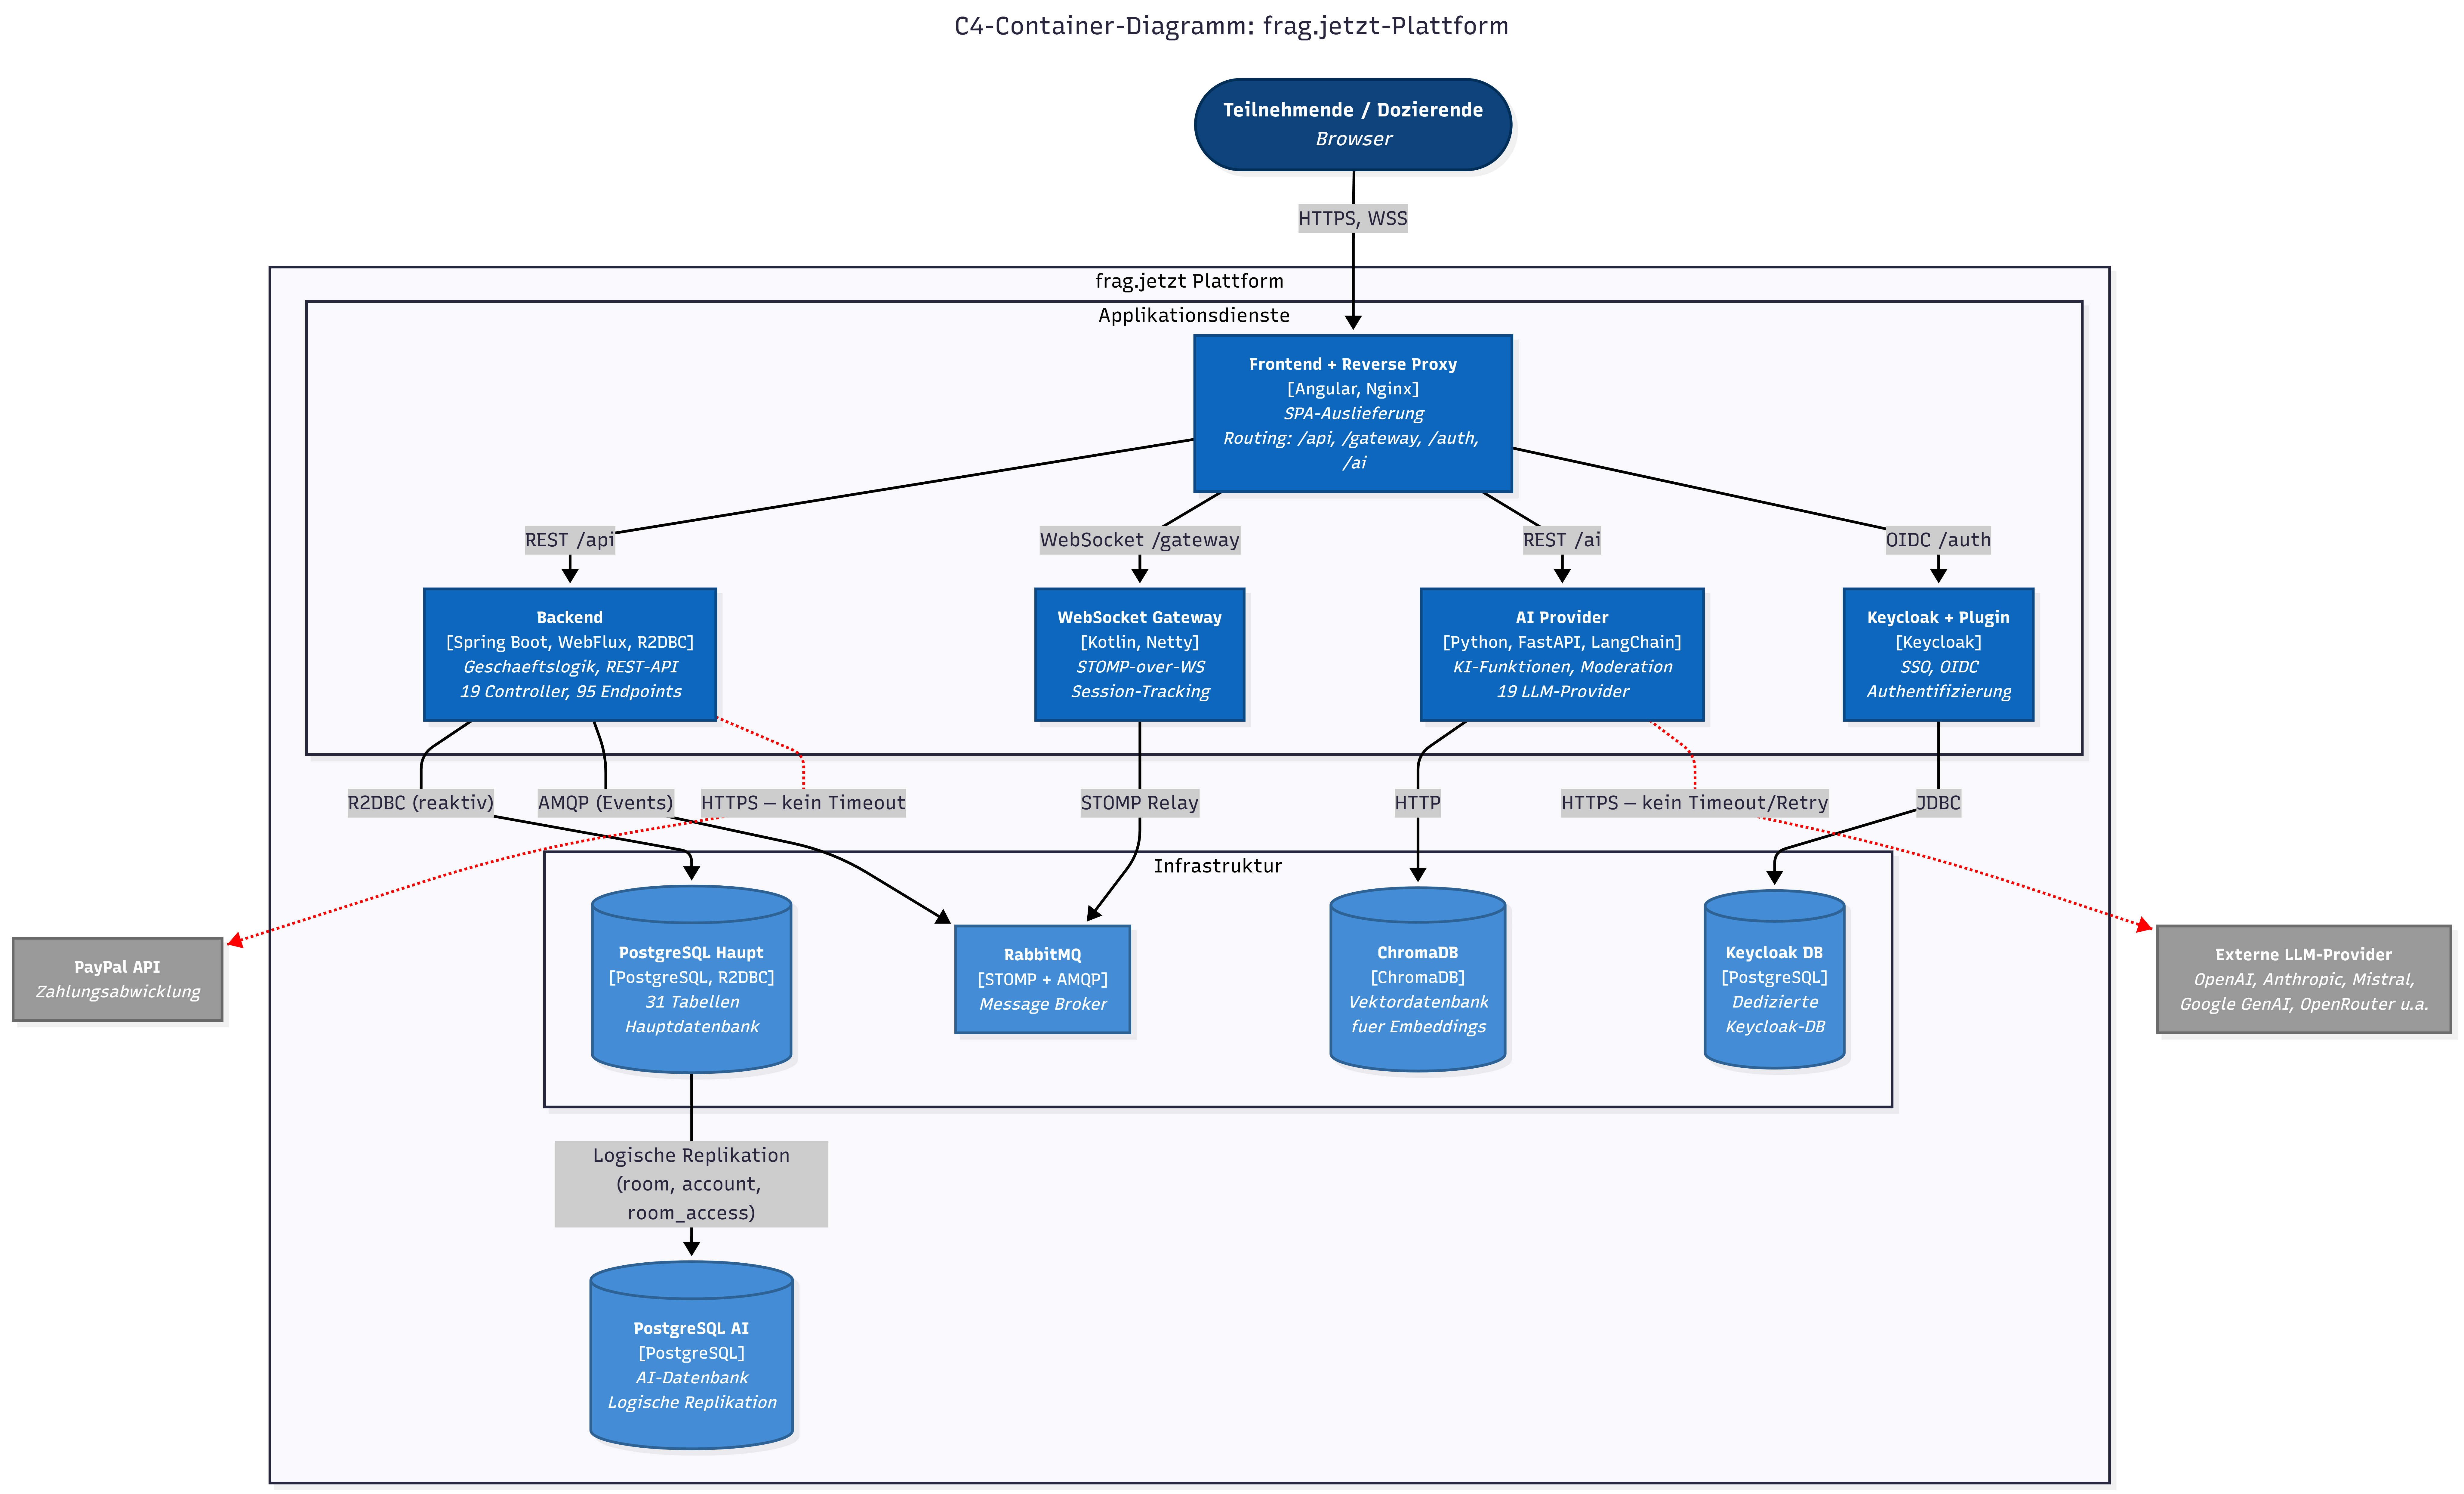
\includegraphics[angle=90,height=0.75\textheight,keepaspectratio]{images/frag.jetzt C4-Container-Diagram.png}
\caption{C4-Container-Diagramm der frag.jetzt-Architektur in Vollseitenansicht}
\label{fig:c4-fragjetzt-architektur-vollseite}
\end{figure}
